%Chaotic systems, when visualised, often exhibit complex patterns due to their non-linear behaviour. These objects can loosely be defined as fractals\footnote{There are many definitions for what a fractal is. Mandelbrot defines them as (...)}, and we can measure how complicated one fractal is compared to another. Though our notion of chaos is not necessarily relevant in this section, fractal dimension will be used to measure the complexity of chaotic systems in further sections.%

%Fractal dimension can be summarised as the measure of an object's complexity or detail. Unlike the dimension of standard objects, fractal dimensions can take non-integer values. This allows objects in the same space to be compared in terms of how complicated their shape is. There are multiple ways to calculate or approximate an object's fractal dimension%
When studying dynamical systems that exhibit chaotic behaviour, we often choose to reduce them to a simpler form in order to obtain quantifiable properties. One key property we look for is \emph{fractal dimension}, which can be thought of as a set's complexity or detail. It can also be seen as a measure of how an object fills space at small scales. Formally, fractal dimension is an index of sets that characterises their complexity as a ratio of the change in detail to the change in scale \cite{mandelbrot1983fractal}. Unlike the values of dimension we are used to, fractal dimension can take non-integer values to distinguish between two objects that fill the same space but in different ways. For instance, a curve in $\mathbb{R}^2$ with fractal dimension close to one behaves much like a standard curve, while one with a fractal dimension close to two behaves more like a surface, e.g., a space-filling curve\footnote{A \textit{space-filling curve} is a function that can take values across the entirety of a subset of $\mathbb{R}^2$, despite being a (one-dimensional) curve}. Objects with fractal dimension are often generated by chaotic dynamical systems. Intuitively, we suspect that these distinctions are in close relation to the degree of sensitivity a system has to its initial conditions, which could imply a connection between fractal dimension and Lyapunov exponents. We can reduce a dynamical system to the set of points that its trajectories tend toward and find the fractal dimension of this set, giving us an idea of how the system behaves.

\section{Fractals}
There are many definitions for what a fractal really is, many of which are not rigorous and can only be applied in specific cases. Our definition will be that of Benoît Mandelbrot's.
\begin{defn}
    Let $X$ be a set. We say that $X$ is a fractal if its fractal dimension strictly exceeds its topological dimension. \cite{mandelbrot1983fractal}
\end{defn}
In this report, the term `topological dimension' will be equal to the standard Euclidean dimension we expect of objects. We have been vague in introducing the notion of non-integer values of dimension; this is because different methods of calculating fractal dimension are used depending on the context of the object. We will introduce these methods after the different contexts are clear.

\section{Self-Similarity and the Mass-Scaling Factor Method}
Our first context is one which is often used as a definition for fractals; that is, self-similar objects. Intuitively, \emph{self-similar} objects are those that are made up of smaller copies of themselves, such as a solid cube. We see a sense of self-similarity in nature, so fractals are often exemplified as, say, the branches of a tree. While fascinating, this notion of self-similarity will not be relevant in our case. We will see sets that are infinitely perfectly self-similar as they have been defined to be this way by an unbounded recursive construction.

While a little more abstract, the fractal dimensions of objects that exhibit self-similarity can be calculated in a simple way. The following method is motivated by translating our usual notions of an object's dimension to that of fractal dimension, in order to better understand what we are working with. 

\begin{prop} \label{MSF}
    (The mass-scaling factor method)
    \begin{enumerate}
        \item Say some self-similar object has a mass equal to one.
        \item Within the object, find a section that is an identical copy of the original.
        \item Comparing the copy to the original, work out the mass $m$ and scaling factor $s$ of the copy (this should be clear for simple self-similar shapes).
        \item Let $M=1/m$ and $S=1/s$. The fractal dimension $D$ of the object is then $S^D=M.$ Equivalently, $D=\log{_SM}$
    \end{enumerate}
\end{prop}
%\begin{defn}
    %The \textbf{scaling factor}, $S$ of a self-similar object is the ratio in size between itself and the `first' copy of itself.
%\end{defn}

%\begin{defn}
    %Suppose a self-similar object has `mass' equal to one. The \textbf{mass scaling factor}, $M$, of the object is the ratio between the masses of the object and the first copy of itself.
%\end{defn}
%\textbf{What do we mean by mass?}
%\begin{defn}
    %The \textbf{fractal dimension} of an object is the real number, $D$, such that $$S^D=M.$$ Equivalently, $$D=\log{_SM}$$
%\end{defn}
This definition of an object's dimension satisfies our usual methods of determining dimension; using elementary intuition, we can see that a straight line, a square, and a cube have fractal dimensions one, two, and three, respectively. In fact, the idea of dimension being a measure of how an object fills space has always been true for normal notions of dimension; scaling down a cube by some factor reduces its mass by that factor to the power of three, which is the dimension of the cube. As expected, this means they are not fractals due to the fractal dimension being equal to the topological dimension. However, what we have now is a distinction between, say, two curves in $\mathbb{R}^2$ or two surfaces in $\mathbb{R}^3$, where the higher fractal dimension points towards a more detailed structure.
%\begin{exmp}
    %The `Koch curve' is constructed by repeatedly adding triangular bumps to the centre-thirds of a line, starting with a straight line of unit length.
    
    %If we take a straight line and the Koch curve embedded in $\mathbb{R}^2$, both are continuous curves, so they are of the same dimension in the usual sense; however, we will see that the fractal dimensions are not equal due to the Koch curve being more complex. 
    %\begin{figure}
        %\centering
        %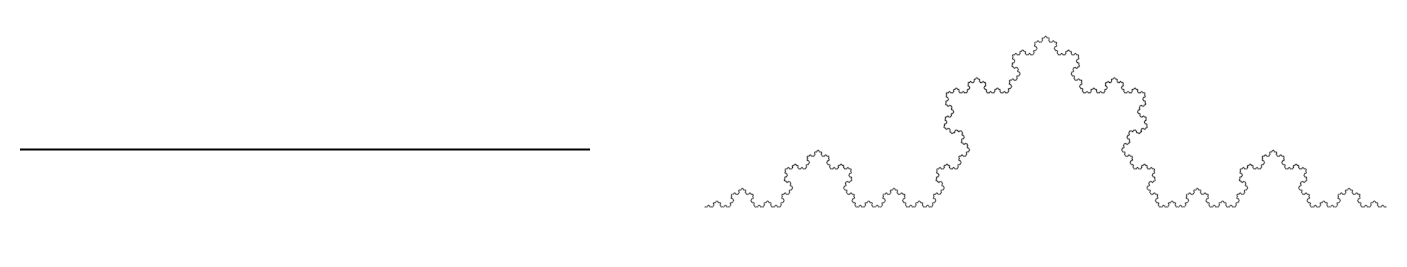
\includegraphics[width=0.8\linewidth]{Images/Koch.png}
        %\caption{Straight line and Koch Curve}
       % \label{fig:enter-label}
    %\end{figure}
    %Both are self-similar, since any cut of a line is similar to the line and the Koch curve splits into four identical copies of itself, each of which is scaled down in size by $1/3$. It is clear that, taking any cut of the straight line, say $1/a^{th}$ of it, gives a line of mass $1/a$, so we have that the line has a scaling factor equal to its mass-scaling factor, giving a fractal dimension of one, as we would expect. For the Koch curve, we have a scaling factor of $1/3$, since each copy of itself is $1/3^{rd}$ the length of the original and a mass-scaling factor of $1/4$, since we have four copies of this size. Therefore, we have that the fractal dimension of the Koch curve is given by the value of $D$ such that
    %$$\frac{1}{3}^D=\frac{1}{4},$$
    %equivalently, such that
    %$$3^D=4.$$
    %Therefore,
    %$$D=\log{_34}\approx1.26186.$$
    %This means that the Koch curve is a fractal, since its fractal dimension is strictly greater than its topological dimension which, being a curve in the plane, is one.
%\end{exmp}

\begin{exmp} \label{exmp2.3}
    The `Koch curve', pictured in Figure \ref{fig:Koch}, is constructed in the following way. Take a straight line segment embedded in $\mathbb{R}^2$ and remove the middle third and replace it with an `equilateral-triangle bump'. Note there are now four straight lines of length $1/3$ of the original. On each new straight line, add equilateral-triangle bumps to their middle thirds and repeat. At each stage, each quarter of the curve is an identical copy of the last version, scaled down by $1/3$.
    \begin{figure}
        \centering
        
\includegraphics[width=1\linewidth]{Images/Koch new.png}
        \caption{Construction of the Koch curve from a straight line, showing the first, second and fifth iterate. In blue are the sections of the Koch curve that are scaled copies of the iterate before it.}
        \label{fig:Koch}
    \end{figure}
    Let us follow the steps in Proposition \ref{MSF} to determine the fractal dimension of the Koch curve:
    \begin{enumerate}
        \item We say the Koch curve has mass and length one.
        \item Considering the curve after infinite iterates, each quarter of the curve is identical to the entire thing.
        \item Since each quarter of the curve is a copy of the original scaled down by $1/3$, one copy has mass $m=1/4$ and scaling factor $s=1/3$.
        \item We have $M=1/(1/4)=4$ and $S=1/(1/3)=3$, so the fractal dimension of the Koch curve is $D=\log_34\approx1.26186$
    \end{enumerate}
    Since the Koch curve is a continuous curve in $\mathbb{R}^2$, its topological dimension is one. Therefore, we have that the Koch curve is indeed a fractal, as its fractal dimension strictly exceeds its topological dimension.
\end{exmp}
%From the example above, we can see that we have a measurable value that will distinguish shapes based on their complexity. This will prove useful in chaos theory as knowing the fractal dimension of an object then allows us to talk about measures, which will be affected by the complexity of objects. The issue will be for objects that are not so simply defined and do not exhibit self-similarity. For this, we will need another method for calculating fractal dimension%.
We see here, a glimpse of what an object's fractal dimension is, with the restriction that our method only works in the case of perfect self-similarity. We have another method that does not depend on this property; however, the context in which it is used must first be introduced.
\section{Attractors and the Box-Counting Method}
We often want to look for the points that dynamical systems tend toward as time progresses. 
In our models, the existence and uniqueness theorem tells us that these points are deterministic in that fixed initial conditions will grant the same result every time. 
For stable systems, we can further say that some small perturbation of the initial conditions will not greatly affect the solution; this allows us to make strong predictions about how the system will evolve over time. 
With this in mind, we naturally arrive at the definition of an \emph{attractor}, the set of points in which a system evolves toward over time and then stays there forever. 
A key property of attractors is that they do not change under a small perturbation of initial conditions; trajectories of nearby points eventually fall into the same set of points. \cite{feldman2012chaos}

%\begin{defn}
    %An \textbf{attractor}, $\mathbf{X}  \in \mathbb{R}^n$, of an $n$-dimensional dynamical system, $F(\mathbf{x},t)$, is the set of points $\mathbf{x}_\infty\in\mathbb{R}^n$ that the trajectory of an initial point $\mathbf{x_0}$ tends toward $t\to\infty$.
    %$$\mathbf{X} := \{\mathbf{x}_\infty\in\mathbb{R}^n:F(\mathbf{x_0},t)\to\mathbf{x}_\infty \text{ as } t\to \infty\},$$
    %such that points in some small neighbourhood of %$\mathbf{x_0}$ will share the same attractor%.%
%\end{defn}%

%\begin{defn}
    %Let $F(\mathbf{x},t)$ be an $n$-dimensional dynamical system and $\mathbf{x_0}$ be some initial point. An \textbf{attractor}, $\mathbf{X}  \in \mathbb{R}^n$ of $\mathbf{x_0}$ is the set of points
    %$$\mathbf{X} := \{\mathbf{x}\in\mathbb{R}^n:F(\mathbf{x_0},t) = \mathbf{x}\},$$
    %such that the trajectories are dense near these points after some large $t$. Furthermore, points in some small neighbourhood of $\mathbf{x_0}$ share the same attractor.
%\end{defn}

%\begin{defn}
    %Let $F(\mathbf{x},t)$ be an $n$-dimensional dynamical system and $\mathbf{x_0}$ be some initial point. An \textbf{attractor}, $\mathbf{X}  \in \mathbb{R}^n$ of $\mathbf{x_0}$ is the set of points such that:
    %\begin{enumerate}
        %\item the trajectory remains dense in after some large number of iterations; and
        %\item points in some small neighborhood of $\mathbf{x_0}$ share the same attractor.
    %\end{enumerate}. 
%\end{defn}
%For simpler stable systems, we can find formulas for defining these sets by taking derivatives of the map $F$ and finding the stable points.

For stable systems, two types of attractors are: fixed points, a state of equilibrium; and limit cycles, a set of points that the system will eventually stay in, periodically, forever. 
%Since we have a set of distinct points in $\mathbb{R}^n$, we say these attractors are one-dimensional. 
%Small changes to the initial conditions will have a small effect on the attractors for stable systems. If we alter the parameters of a given system, we can see changes in stability as well as changes in the attractor type. 

%Given a system that is not stable, the trajectories may diverge. In a confined space, we have the example of a fluid mixing in a box, and we say that the attractor of this system is the whole three-dimensional space.
For chaotic systems, things are different. Since we have a strong sensitivity to initial conditions, even stable points can become unstable at the slightest perturbation due to the existence of a positive Lyapunov exponent. This means we cannot define the set so easily since a minor change to one initial point could greatly affect its outcome over time. This being said, we may not have complete divergence, since we can plot the trajectories after a high number of iterations and still see a distinct set. Furthermore, zooming in to these attractors, we see that they can take the form of fractals. 

These properties have coined the term `strange' attractors since they paradoxically show convergence of a system that seems to never settle down. Thus the term \emph{strange attractor} describes attractors that have a fractal structure and are those of dynamical systems that observe a sensitive dependence on initial conditions \cite{feldman2012chaos}. To better understand strange attractors, a staple example is the Hénon map, a simplified section of the famous Lorenz system \cite{nonlinear_system}.
\begin{exmp}
    We define the Hénon map, which acts on points $(x,y)\in \mathbb{R}^2$, as the two-dimensional discrete-time dynamical system,
\begin{equation}
    x_{n+1} = 1 - a x_n^2 + y_n, \quad y_{n+1} = b x_n.   
\end{equation}\label{Henonequation}
The classic parameters are $a=1.4$ and $b=0.3$, with which the map is chaotic. Plotting the trajectory of the initial point $(0,0)$ gives us a prime example of a strange attractor.
    \begin{figure}
        \centering
        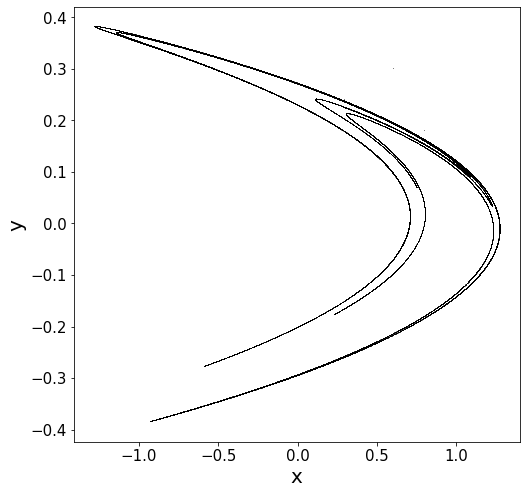
\includegraphics[width=0.4\linewidth]{Images/Henon attractor.png}
        \caption{$100,000$ iterations of the Hénon map with initial point $(x_0, y_0)=(0,0)$.}
        \label{fig:Henon1}
    \end{figure}
    We see the set of points this system attains as the nested curves in Figure \ref{fig:Henon1}. It is important to understand these curves are made up of distinct points, given by each iteration of the Hénon map, and these points are by no means following the curves continuously; we see that the 95th through 99th iterations\footnote{Choosing the 95th through 99th iterations was completely arbitrary in the interest of a diagram that represented the point well. Almost any iterations would have shown the sensitive dependence on initial conditions.} are far apart from each other and follow no obvious pattern. Changing the initial conditions by a small amount, the attractor remains similar, but these same iterations appear in drastically different positions on it, alluding to the chaotic nature of this system. This behaviour can be seen in Figure \ref{fig:Henon2}.
    \begin{figure}
        \centering
        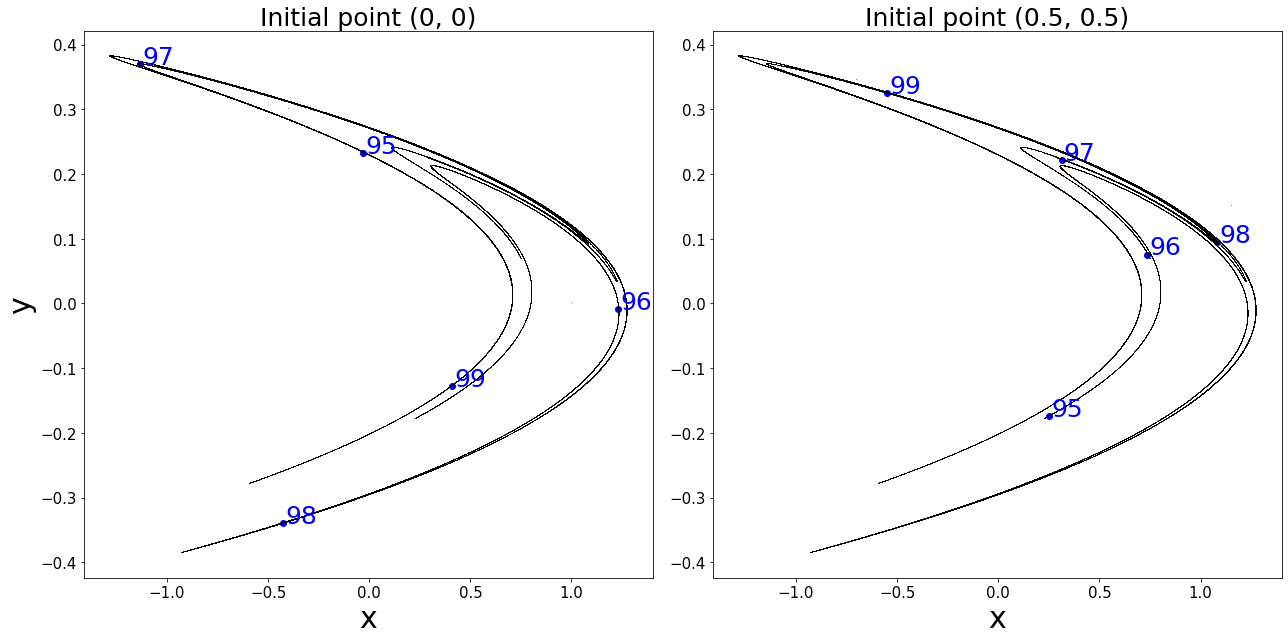
\includegraphics[width=0.75\linewidth]{Images/Henon attractor with labels.png}
        \caption{The Hénon attractor, generated from two different initial points, $(x_0,y_0) = (0,0)$ and $(x_0',y_0') = (0.5,0.5)$. The attractor is identical for both initial points while the system itself appears to be chaotic due to the iterates following drastically different trajectories.}
        \label{fig:Henon2}
    \end{figure}
    The fact that a similar attracting set exists for both initial points indicates this is an attractor by definition.
    Zooming into a section of it will show more self-similar curve, as shown in Figure \ref{fig:Henon3}, is another evidence of it being a strange attractor. 
    \begin{figure}
        \centering
        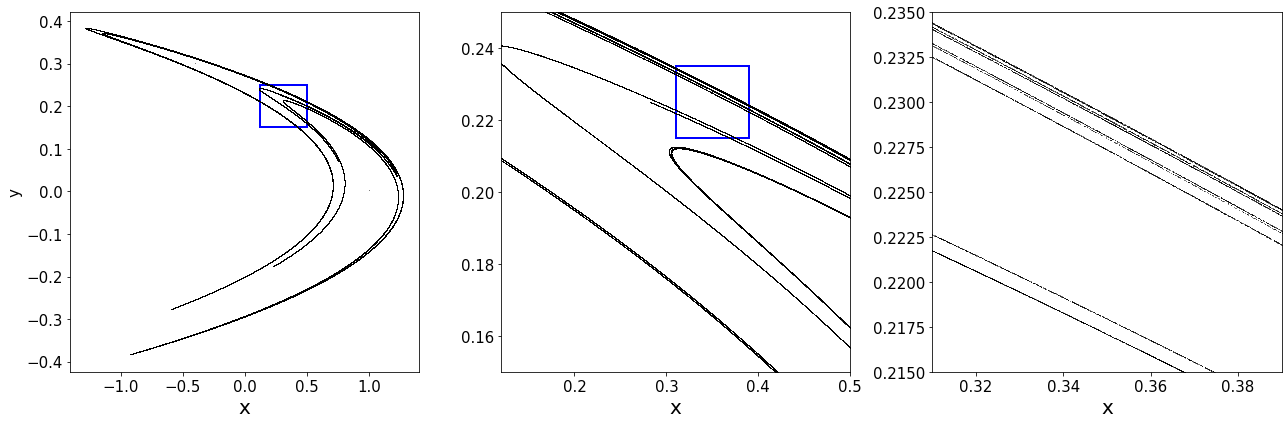
\includegraphics[width=1\linewidth]{Images/henon zoom.png}
        \caption{Zooming in to the blue boxes on the Hénon attractor to see the fractal structure of the object.}
        \label{fig:Henon3}
    \end{figure}
    Since the attractor has a fractal structure and its system has a sensitive dependence on initial conditions, we conclude that this is indeed a strange attractor.
\end{exmp}
From this example, it is clear that the mass-scaling factor method of determining fractal dimension will no longer be of use, since we cannot simply find a smaller version of the Hénon map inside itself, let alone determine its mass-scaling factor. However, the idea of how the attractor fills space will motivate a new method for approximating the value.

Motivated by the need for a universal method for calculating fractal dimension, the following method can be used to approximate the fractal dimension of any object in some subset of $\mathbb{R}^n$. The idea is, given some fractal object, we measure the amount of space it fills as we zoom into its structure. We do this by overlaying a grid of $n$-dimensional boxes over the object and counting how many boxes it is contained in. We then decrease the size of the boxes and count again, repeating this process a number of times. With the results, we plot the logarithms of the number of boxes against the size of the boxes and take the slope of best fit to be the fractal dimension. Explicitly, we have a formula
\begin{equation}
    D = \lim_{\epsilon \to 0} \frac{\log N(\epsilon)}{\log(1/\epsilon)},
\end{equation}\label{boxcountingD}
where $\epsilon$ is the size of each box (length of one side of each $n$-cube) and $N(\epsilon)$ is the number of boxes that the object is contained in for each $\epsilon$. For complicated objects, the best way to do this is by use of computer code that will do this whole process to a strong level of accuracy. It must be noted that Formula \ref{boxcountingD} may not be valid in practice since, in Python, it is only realistic to plot a finite number of points of the attractor. Therefore, we must be careful to fashion code that suits the attractor we are working with, or else the box-count can `bottom-out' once the boxes become too small, giving a skewed gradient. With this in mind, we return to the previous example to calculate the fractal dimension of the Hénon attractor by the box-counting method.
\begin{exmp}\label{henonboxex}
    Using Python, we calculate the fractal dimension of the Hénon attractor by following the box-counting method. The code overlays a grid of boxes over the fractal and counts the number of boxes that contain it as the box size decreases. In Figure \ref{fig:Henon4}, we see some blue boxes that contain the attractor as their size decreases.
    \begin{figure}
        \centering
        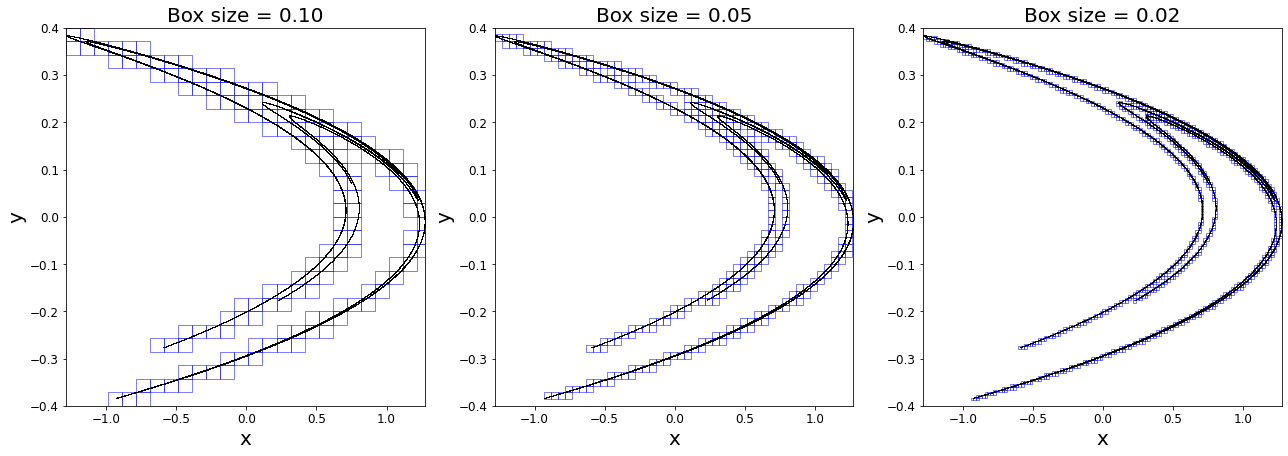
\includegraphics[width=1\linewidth]{Images/Henon boxes.png}
        \caption{Blue squares are those from the grid that contain at least one iterate of the Hénon attractor after $10,000,000$ iterations, using initial point $(0,0)$. The first $10,000$ iterates are discarded to remove any `dust' for accuracy.}
        \label{fig:Henon4}
    \end{figure}
    The code then plots $\log (N(\epsilon))$ against $\log (1/\epsilon)$ for many values of $\epsilon$ and finds the line of best fit through the points on the plot. The gradient of the line is then calculated to achieve a value for $D$. This is all given in Figure \ref{fig:Henon5}.
    \begin{figure}
        \centering
        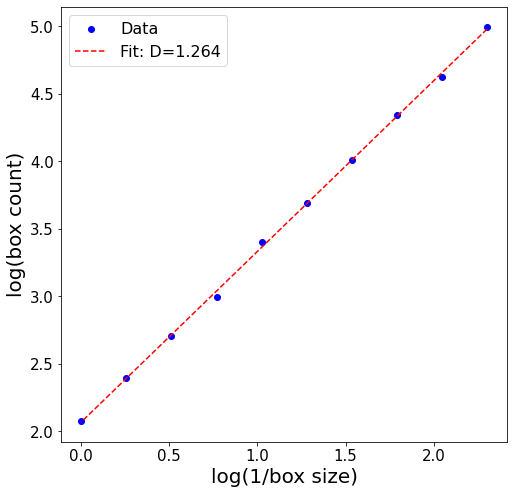
\includegraphics[width=0.5\linewidth]{Images/henon loglog.png}
        \caption{$\log (N(\epsilon))$ as a function of $\log(1/\epsilon)$ for ten values of $\epsilon$ and the line of best fit through the data points which has gradient equal to the fractal dimension of the Hénon attractor.}
        \label{fig:Henon5}
    \end{figure}
    From the gradient of the line, we get a value of $D\approx1.264$, which is our fractal dimension of the Hénon attractor by the box-counting method. The code written for this example is shown in Appendix \ref{boxalg}.
\end{exmp}
With this, we have a more versatile method for calculating the fractal dimension of a fractal object in $\mathbb{R}^n$. We find one more method for fractal dimension calculation by returning to Section \ref{LyapCts}.


\section{The Kaplan–Yorke Conjecture}

The Lyapunov spectrum, as discussed in Section \ref{LyapCts}, is closely related to the fractal dimension of the attractor. The Kaplan–Yorke conjecture uses Lyapunov exponents to deduce the dimension of an attractor within a dynamical system.
%In order to quantify the complexity of chaotic attractors, which often exhibit fractal structure, Lyapunov exponents can help provide information about the system's dynamics, while fractal dimension characterises the geometry of the attractor.
The conjecture is able to link these two concepts together, which is based on the idea that the sum of Lyapunov exponents relates to the expansion and contraction rates of phase space volumes. 
The fractal dimension is then estimated by balancing the cumulative expansion (positive Lyapunov exponents) against the cumulative contraction (negative Lyapunov exponents). 
Let us arrange the Lyapunov exponents from largest to smallest such that $\lambda_1 \geq \lambda_2 \geq \dots \geq \lambda_n$. Let $k$ thus be the largest index in which
\begin{align}
    \sum_{i=1}^k \lambda_i\geq 0 \quad\quad \text{ and } \quad \quad \sum_{i=1}^{k+1} \lambda_i <0 \label{eq:criteria}
\end{align}

We then have the Kaplan-Yorke dimension \cite{Peitgen1992}, defined as
\begin{align}
    D = k + \frac{\sum_{i=1}^k \lambda_i}{|\lambda_{k+1}|},\label{Kaplan-Yorke}
\end{align} 
where $k$ is the largest integer such that $\sum_{i=1}^k \lambda_i \geq 0,$ which provides an estimate of the fractal dimension. We return once more to the example of the Hénon Map to calculate its Kaplan-Yorke dimension.

\begin{exmp}
    When we compute the Lyapunov exponent for the Hénon Map \eqref{Henonequation} using Section \ref{LyapCts}, we attain the values approximated by the graphs in Figure \ref{fig:LyaHen}.
    \begin{figure}
        \centering
        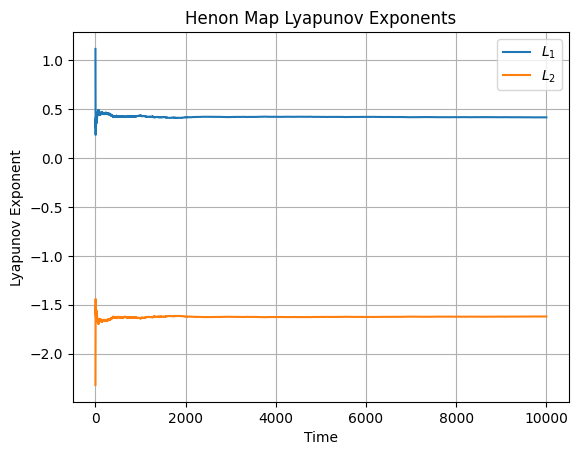
\includegraphics[width=0.8\linewidth]{Bifurcation Images/lyapunov_henon.png}
        \caption{Lyapunov exponents for the Hénon Map with initial conditions of $(x,y)=(0.1,0.1)$ where $a=1.4$ and $b=0.3$. The exponent $\lambda_1$ after several iterations of time is seen to be greater than 0 implying that the system is chaotic under the initial conditions.}
        \label{fig:LyaHen}
    \end{figure}
    The Lyapunov exponents for the Hénon map were computed to be 
    \begin{align*}
        \lambda_1 &= 0.41762663136121125, \\
        \lambda_2 &= -1.6215994356871315,
    \end{align*}
     when we used \eqref{eq:lyapunov_cont}. However if we use \eqref{eq:continuous}, we get the exponents to be 
    \begin{align}
        \lambda_1 &= 0.6025078700079933, \label{henon_ly} \\
        \lambda_2 &= -2.339473464174202. \label{henon_lypn}
    \end{align}
    Using \eqref{henon_ly} and \eqref{henon_lypn}, then from \eqref{eq:criteria}, we can observe that our value for $k$ must be 1. Thus when we substitute these values into \eqref{Kaplan-Yorke},
    \begin{align*}
        D &= 1 + \frac{\sum_{i=1}^1 \lambda_i}{|\lambda_{2}|} \\
        &=1 + \frac{0.6025078700079933}{|-2.339473464174202|} \\
        &=1.257539946.
    \end{align*}
    This gives us that the fractal dimension of the Hénon attractor by the Kaplan–Yorke conjecture is $D=1.257\dots$, which aligns very closely to the result found in Example \ref{exmp2.3}. This provides evidence for the conjecture's validity and shows there could be some connection between fractal dimension and Lyapunov exponents, as suspected.

We now have a range of methods to calculate fractal dimension, giving an index of fractals distinguished by their small-scale complexity. 
This complexity and these fractal shapes are seen throughout nature as a characteristic of what we consider to be a natural-looking shape\footnote{“Clouds are not spheres, mountains are not cones, coastlines are not circles, and bark is not smooth, nor does lightning travel in a straight line.”
― Benoît Mandelbrot \cite{mandelbrot1983fractal}}.
Noticing this, there have been a number of fascinating applications of fractal geometry. For one, computer-image generation uses fractals to create shapes that look natural, such as mountain ranges, plants, and coastlines. Without fractals, we could do our best to draw the detailed ridge of a mountain range from a given distance away, but the detail would not remain as we move closer. Fractals allow us to generate this detail to any scale; which, in the interest of realistic simulation, makes for a much better representation of such objects. The fractals we use depend on what we are trying to model; mountain ranges, plants, and coastlines all have different ranges of fractal dimensions that best represent their real-life structure. \cite{Haeseler2012}
\end{exmp}

%\section{Fractal Dimension Implications}
%For chaotic dynamical systems, we can now quantify the dimension of the attractors with values that better represent the strange structure they can have. These values give us an idea of the properties of the system itself.\\

%First, the higher the fractal dimension, the more an attractor of a system fills the space it occupies. In an $n$-dimensional subset of $\mathbb{R}^n$, this means that an attractor with a fractal dimension close to $n$ will be associated with a system that has a higher number of effective degrees of freedom.
%In particular, suppose we are working in some subset of $\mathbb{R}^2$. We have, on one extreme, that the attractor of the system is a single fixed point, where we would have a zero-dimensional attractor. On the other extreme, the attractor is the whole space, two-dimensional. A one-dimensional attractor would be one that takes the form of a smooth continuous curve\footnote{For discrete time systems, an attractor in the shape of a smooth curve will not be continuous in $\mathbb{R}^2$ but the box-counting dimension will still be equal to one.}. An attractor's fractal dimension then tells us how chaotic a system is; whether it behaves more like a fixed point or limit cycle, alluding to a system that is close to being stable; fills nearly the entire subspace, much like fluid mixing in a box; or it takes values across a set similar to a smooth curve, like the Hénon attractor.  How close the fractal dimension is to the integer values generally points towards how strong the attractor is, i.e., how long it takes for nearby points to get within a small distance of the attractor. This correspondence gives a good insight into the stability of attractors as the system's parameter changes. A case we will look into extensively is when we plot a \textbf{bifurcation diagram} of a one-dimensional discrete-time dynamical system, which gives a visual representation of how the attractors change as we vary a parameter. The \textbf{bifurcation points} (where the attractor type changes, doubling the period of a limit cycle each time) are surrounded by `dust' which is made by thousands of iterations taking a long time to settle around the attractor and other nearby attractors. These points have attractors that are technically fixed points or limit cycles, so should intuitively have a dimension of zero. However, the iterates converge asymptotically to this attractor so, plotting any large finite number of iterates, the attractor takes the form of a line in one-dimension; the fractal dimension of the attractor tends toward one. This tells how weakly stable these points are, leading to issues of numerical calculation around these points. On the other hand, we have \textbf{super-stable points} across the bifurcation diagram, that stay at the first iteration forever; fixed points that take no time to settle down, so have fractal dimension exactly zero. These points will be of great interest to us since numerical approximations of these points will be a key step in deriving Feigenbaum's universal constants.\\

%Varying the parameters of some system, we see changes in the types of attractor as well as fractal dimension. What this means is that there are significant parameter values in which the type of attractor changes or the fractal dimension reaches value we take interest in. Throughout this report, we look at one-dimensional discrete time dynamical systems and take great interest in the changes we see to the attractors as we alter the system's parameters. We witness a phenomenon called \textbf{bifurcation} in which a fixed point attractor becomes a period-two limit cycle, period-two becomes period-four, and so on, the period doubling each time bifurcation occurs. This change occurs at specific values of the system's parameters, called the \textbf{bifurcation points}. These points are so weakly stable that 

%An interesting case is when an object has an integer-valued fractal dimension that is higher than expected. For example, a curve in $\mathbb{R}^2$ can be so complex that it has a fractal dimension equal to two, without needing to be a space-filling curve. What this means is we can zoom into the curve at any scale and find incredible detail. These objects are important to chaos theory as they provide an intriguing and beautiful advertisement for the subject.